\documentclass[letterpaper, 11pt]{extarticle}
% \documentclass{article}
% \usepackage{fontspec}

% ==================================================

% document parameters
% \usepackage[spanish, mexico, es-lcroman]{babel}
\usepackage[english]{babel}
\usepackage[margin = 1in]{geometry}

% ==================================================
\usepackage{kotex}
\usepackage{listing}
\usepackage{listings}
% Packages for math
\usepackage{mathrsfs}
\usepackage{amsfonts}
\usepackage{amsmath}
\usepackage{amsthm}
\usepackage{amssymb}
\usepackage{physics}
\usepackage{dsfont}
\usepackage{esint}

% ==================================================

% Packages for writing
\usepackage{enumerate}
\usepackage[shortlabels]{enumitem}
\usepackage{framed}
\usepackage{csquotes}

% ==================================================

% Miscellaneous packages
\usepackage{graphicx}
\usepackage{float}
\usepackage{tabularx}
\usepackage{xcolor}
\usepackage{multicol}
\usepackage{subcaption}
\usepackage{caption}
\captionsetup{format = hang, margin = 10pt, font = small, labelfont = bf}

% Citation
\usepackage[numbers,sort&compress]{natbib}

% Hyperlinks setup
\usepackage{hyperref}
\definecolor{links}{rgb}{0.36,0.54,0.66}
\hypersetup{
   colorlinks = true,
    linkcolor = black,
     urlcolor = blue,
    citecolor = blue,
    filecolor = blue,
    pdfauthor = {Author},
     pdftitle = {Title},
   pdfsubject = {subject},
  pdfkeywords = {one, two},
  pdfproducer = {LaTeX},
   pdfcreator = {pdfLaTeX},
   }
\usepackage{titlesec}
\usepackage[many]{tcolorbox}

% Adjust spacing after the chapter title
\titlespacing*{\chapter}{0cm}{-2.0cm}{0.50cm}
\titlespacing*{\section}{0cm}{0.50cm}{0.25cm}

% Indent 
\setlength{\parindent}{0pt}
\setlength{\parskip}{1ex}

% --- Theorems, lemma, corollary, postulate, definition ---
% \numberwithin{equation}{section}

\newtcbtheorem[]{problem}{Problem}%
    {enhanced,
    colback = black!5, %white,
    colbacktitle = black!5,
    coltitle = black,
    boxrule = 0pt,
    frame hidden,
    borderline west = {0.5mm}{0.0mm}{black},
    fonttitle = \bfseries\sffamily,
    breakable,
    before skip = 3ex,
    after skip = 3ex
}{problem}

\tcbuselibrary{skins, breakable}

% --- You can define your own color box. Just copy the previous \newtcbtheorm definition and use the colors of yout liking and the title you want to use.
% --- Basic commands ---
%   Euler's constant
\newcommand{\eu}{\mathrm{e}}

%   Imaginary unit
\newcommand{\im}{\mathrm{i}}

%   Sexagesimal degree symbol
\newcommand{\grado}{\,^{\circ}}

% --- Comandos para álgebra lineal ---
% Matrix transpose
\newcommand{\transpose}[1]{{#1}^{\mathsf{T}}}

%%% Comandos para cálculo
%   Definite integral from -\infty to +\infty
\newcommand{\Int}{\int\limits_{-\infty}^{\infty}}

%   Indefinite integral
\newcommand{\rint}[2]{\int{#1}\dd{#2}}

%  Definite integral
\newcommand{\Rint}[4]{\int\limits_{#1}^{#2}{#3}\dd{#4}}

%   Dot product symbol (use the command \bigcdot)
\makeatletter
\newcommand*\bigcdot{\mathpalette\bigcdot@{.5}}
\newcommand*\bigcdot@[2]{\mathbin{\vcenter{\hbox{\scalebox{#2}{$\m@th#1\bullet$}}}}}
\makeatother

%   Hamiltonian
\newcommand{\Ham}{\hat{\mathcal{H}}}

%   Trace
\renewcommand{\Tr}{\mathrm{Tr}}

% Christoffel symbol of the second kind
\newcommand{\christoffelsecond}[4]{\dfrac{1}{2}g^{#3 #4}(\partial_{#1} g_{#2 #4} + \partial_{#2} g_{#1 #4} - \partial_{#4} g_{#1 #2})}

% Riemann curvature tensor
\newcommand{\riemanncurvature}[5]{\partial_{#3} \Gamma_{#4 #2}^{#1} - \partial_{#4} \Gamma_{#3 #2}^{#1} + \Gamma_{#3 #5}^{#1} \Gamma_{#4 #2}^{#5} - \Gamma_{#4 #5}^{#1} \Gamma_{#3 #2}^{#5}}

% Covariant Riemann curvature tensor
\newcommand{\covariantriemanncurvature}[5]{g_{#1 #5} R^{#5}{}_{#2 #3 #4}}

% Ricci tensor
\newcommand{\riccitensor}[5]{g_{#1 #5} R^{#5}{}_{#2 #3 #4}}

\begin{document}

\begin{Large}
	\textsf{\textbf{Project}}
\end{Large}

\vspace{1ex}

\textsf{\textbf{Student:}} \text{Jonghyun Woo}, \href{jhwoo200@gmail.com}{\texttt{jhwoo200@gmail.com}}\\
\textsf{\textbf{Lecturer:}} \text{Seokwon Lee}, \href{seokwonlee@cau.ac.kr}{\texttt{seokwonlee@cau.ac.kr}}

\vspace{2ex}

We want to obtain the optimal control problem.

\begin{equation}\label{eq:ocp1}
	J = u(T)
\end{equation}

Subject to

\begin{equation}\label{eq:ocp2}
	\begin{aligned}
		\dot{x}(t) & = u(t),         \\
		\dot{y}(t) & = v(t),         \\
		\dot{u}(t) & = U \cos \beta, \\
		\dot{v}(t) & = U \sin \beta.
	\end{aligned}
\end{equation}

With initial conditions
\begin{equation}\label{eq:ocp3}
	\begin{aligned}
		x(0) & = 0, \\
		y(T) & = h, \\
		v(T) & = 0.
	\end{aligned}
\end{equation}

\begin{problem}{Problem [1]}{prob1-1}
Formulate the OCP and derive the necessary condition and optimality condition. Solve the above problem by using  embedded solver (GPOPS-II \citep{patterson2014general})
\end{problem}

역학 시스템의 간편한 이해를 위해 상태 변수 $x$, $y$는 위치 $(m)$, $u$, $v$는 속도 $(m/s)$, $U$는 가속도 $(m/s^2)$, control variable $\beta$는 각도 $(rad)$로 정의한다.
위 OCP objective function \eqref{eq:ocp1}은 최종 시간 $T$에서의 속도 $u(T)$를 최소화하는 것으로 정의된다.
위 objective function \eqref{eq:ocp1}은 아래와 같이 재정의할 수 있다.

\begin{equation}\label{eq4}
	\begin{aligned}
		J & = u(0) + \int_{0}^T \dot{u}(\tau) d\tau \\
		  & = u(0) + \int_{0}^T U \cos\beta d\tau
	\end{aligned}
\end{equation}

즉, \eqref{eq4}에서 재정의된 objective function $J$는 초기 속도 $u(0)$와 가속도 $U$에 $\cos \beta$를 곱한 적분의 합으로 정의된다.
이는 $-x$ 방향으로 가하는 힘의 합을 최대화하는 것으로 해석할 수 있다.

GPOPS-II \citep{patterson2014general}를 사용하여 위 OCP를 해결하기 위해서는 초기 시간 $t_0$, 가속도 크기 $U$, 목표 위치 $h$와 같은 OCP 파라미터들을 정의해야 한다.
이를 위해, 아래 표 [\ref{tab1}]에 임의로 정의된 OCP 파라미터들을 정리하였다.

\begin{table}[H]
	\begin{tabular}{|c|c|}
		\hline
		\textbf{Parameters}        & \textbf{Values} \\
		\hline
		Initial time $t_0$         & 0 $(s)$         \\
		\hline
		Acceleration magnitude $U$ & 3 $(m/s^2)$     \\
		\hline
		Target position $h$        & 10 $(m)$        \\
		\hline
	\end{tabular}
	\centering
	\caption{Parameters for the OCP}
	\label{tab1}
\end{table}

또한, GPOPS-II에선 \textbf{boundary condition}을 정의해야 한다.
정의된 boundary condition $x(0)$, $y(T)$, $v(T)$ 외 다른 상태들의 bound는 과한 입력 및 반응을 방지하는 의도로 임의로 설정하였다.
아래 표 [\ref{tab2}]에 boundary condition을 정의하였다.

\begin{table}[H]
	\begin{tabular}{|c|c|c|}
		\hline
		\textbf{Boundary Condition} & \textbf{Lower Bound} & \textbf{Upper Bound} \\
		\hline
		Initial time $t_0$          & 0 $(s)$              & 0 $(s)$              \\
		\hline
		Final time $T$              & 0.01 $(s)$           & 20 $(s)$             \\
		\hline
		Initial state $x(0)$        & 0 $(m)$              & 0 $(m)$              \\
		Initial state $y(0)$        & -20 $(m)$            & 20 $(m)$             \\
		Initial state $u(0)$        & -10 $(m/s)$          & 10 $(m/s)$           \\
		Initial state $v(0)$        & -10 $(m/s)$          & 10 $(m/s)$           \\
		\hline
		Final state $x(T)$          & -20 $(m)$            & 20 $(m)$             \\
		Final state $y(T)$          & $h$ = 10 $(m)$       & $h$ = 10 $(m)$       \\
		Final state $u(T)$          & -10 $(m/s)$          & 10 $(m/s)$           \\
		Final state $v(T)$          & 0 $(m/s)$            & 0 $(m/s)$            \\
		\hline
		Control $\beta$             & $-\pi\,(rad)$        & $\pi\,(rad)$         \\
		\hline
	\end{tabular}
	\centering
	\caption{Boundary conditions for the OCP}
	\label{tab2}
\end{table}

GPOPS-II의 \textbf{guess} structure는 OCP의 초기 상태 $x(0)$, $y(0)$, $u(0)$, $v(0)$와 최종 상태 $x(T)$, $y(T)$, $u(T)$, $v(T)$를 정의한다.
또한, 초기 시간 $t_0$, 최종 시간 $T$, 초기 제어 $\beta$와 적분 term을 정의한다.
표 [\ref{tab3}]에 GPOPS-II의 정의된 guess structure가 정리돼 있다.

\begin{table}[H]
	\begin{tabular}{|c|c|c|}
		\hline
		\textbf{Guess Structure} & \textbf{Values} & \textbf{Description}            \\
		\hline
		Initial time $t_0$       & 0 $(s)$         & Initial time of the OCP         \\
		\hline
		Final time $T$           & 10 $(s)$        & Final time of the OCP           \\
		\hline
		Initial state $x(0)$     & 0 $(m)$         & Initial position in x-direction \\
		Initial state $y(0)$     & 0 $(m)$         & Initial position in y-direction \\
		Initial state $u(0)$     & 0 $(m/s)$       & Initial velocity in x-direction \\
		Initial state $v(0)$     & 0 $(m/s)$       & Initial velocity in y-direction \\
		\hline
		Final state $x(T)$       & 10 $(m)$        & Target position in x-direction  \\
		Final state $y(T)$       & 10 $(m)$        & Target position in y-direction  \\
		Final state $u(T)$       & 0 $(m/s)$       & Final velocity in x-direction   \\
		Final state $v(T)$       & 0 $(m/s)$       & Final velocity in y-direction   \\
		\hline
		Control $\beta$          & 0 $(rad)$       & Initial guess for control angle \\
		\hline
		Integral                 & 0               & Initial guess for integral term \\
		\hline
	\end{tabular}
	\centering
	\caption{Guess structure for the OCP}
	\label{tab3}
\end{table}

그 외, mesh, derivatives, NLP options와 같은 GPOPS-II의 설정을 아래 표 [\ref{tab4}]로 설정하였다.

\begin{table}[H]
    \begin{tabular}{|c|c|}
        \hline
        \textbf{Mesh Settings} & \textbf{Values} \\
        \hline
        Method                 & hp-PattersonRao  \\
        Tolerance              & $1 \times 10^{-6}$ \\
        Max Iterations         & 10               \\
        Col Points Min         & 4                \\
        Col Points Max         & 10               \\
        Phase Col Points       & $4 \times$ones([1, 10]) \\
        Phase Fraction         & $0.1 \times$ones([1, 10]) \\
        \hline
        \textbf{Derivatives Options} & \textbf{Values} \\
        \hline
        Supplier              & sparseFD        \\
        Derivative Level      & second          \\
        \hline
        \textbf{NLP Options} & \textbf{Values} \\
        \hline
        NLP Solver            & ipopt           \\
        NLP Ipopt Options    & linear\_solver = ma57 \\
        NLP Ipopt Options    & tolerance = $1 \times 10^{-10}$ \\
        \hline
    \end{tabular}
    \centering
    \caption{GPOPS-II settings for the OCP}
    \label{tab4}
\end{table}

다음은 GPOPS-II를 사용한 OCP의 solution을 나타낸 것이다.

\begin{figure}[ht]
  \centering
  \begin{subfigure}[b]{0.49\linewidth}
    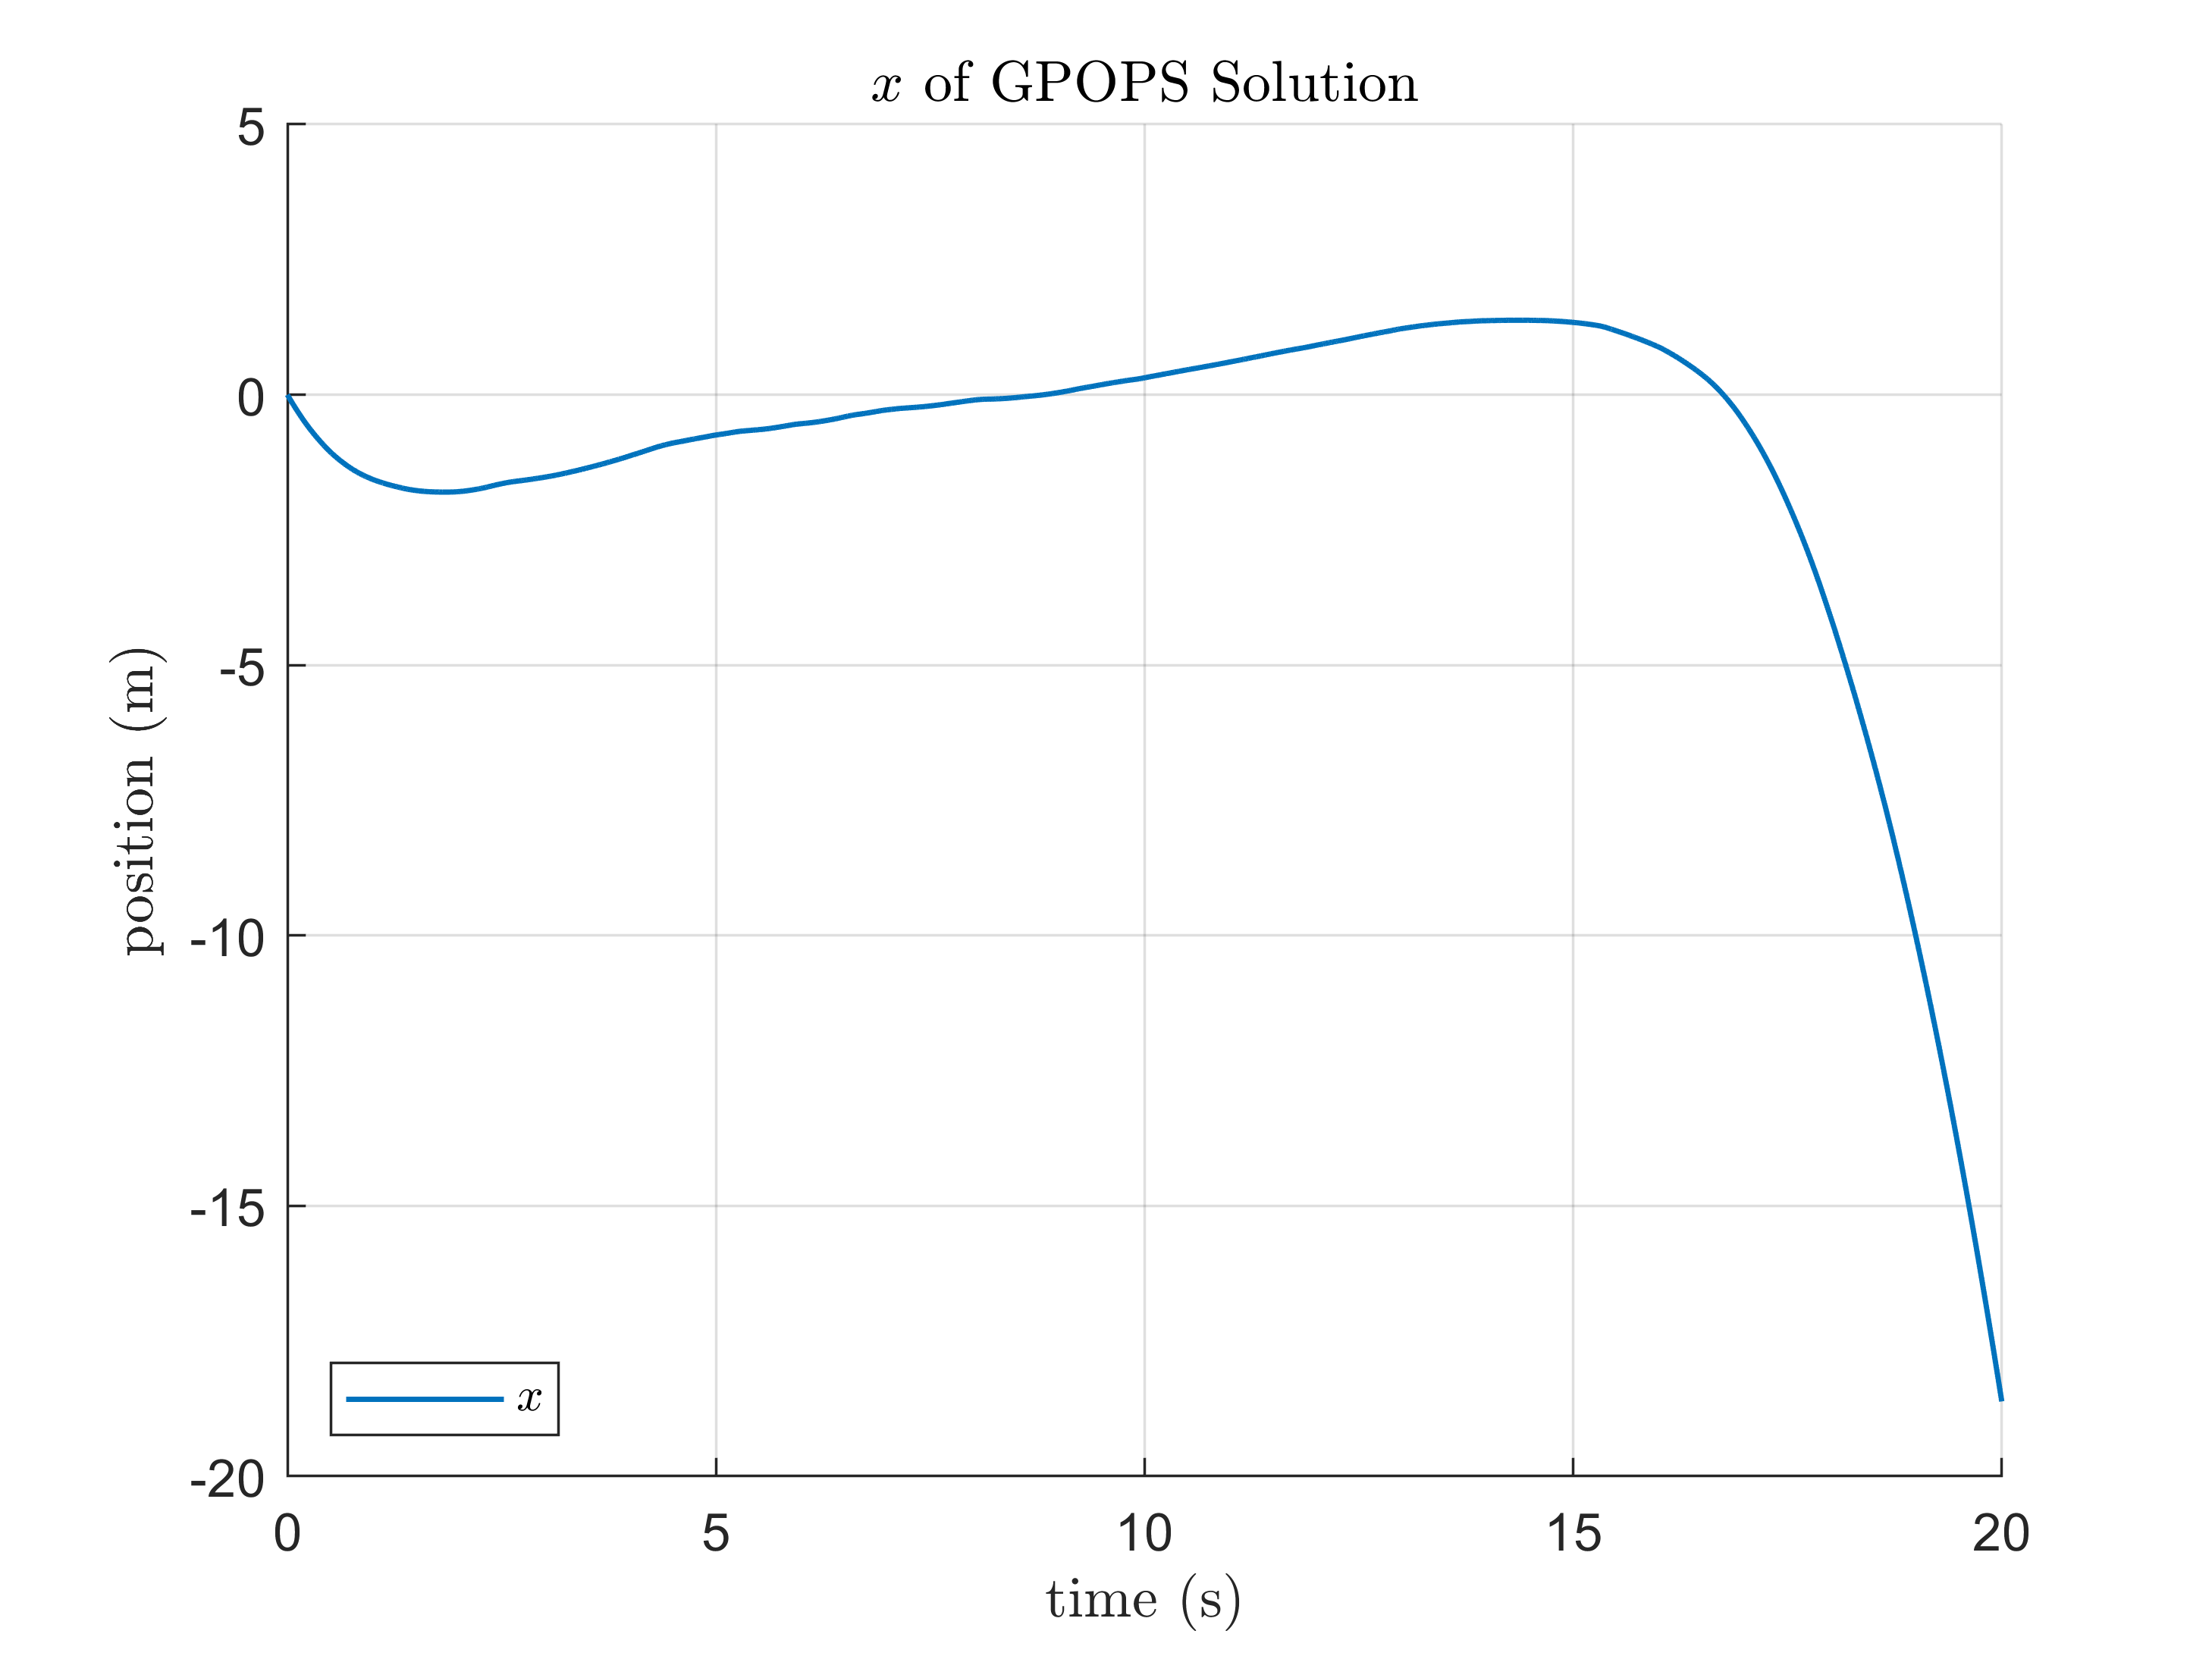
\includegraphics[width=\linewidth]{figures/SolX.png}
    \caption{Position in $x$-direction}
    \label{fig:ocp1_x}
  \end{subfigure}
  \hfill
  \begin{subfigure}[b]{0.49\linewidth}
    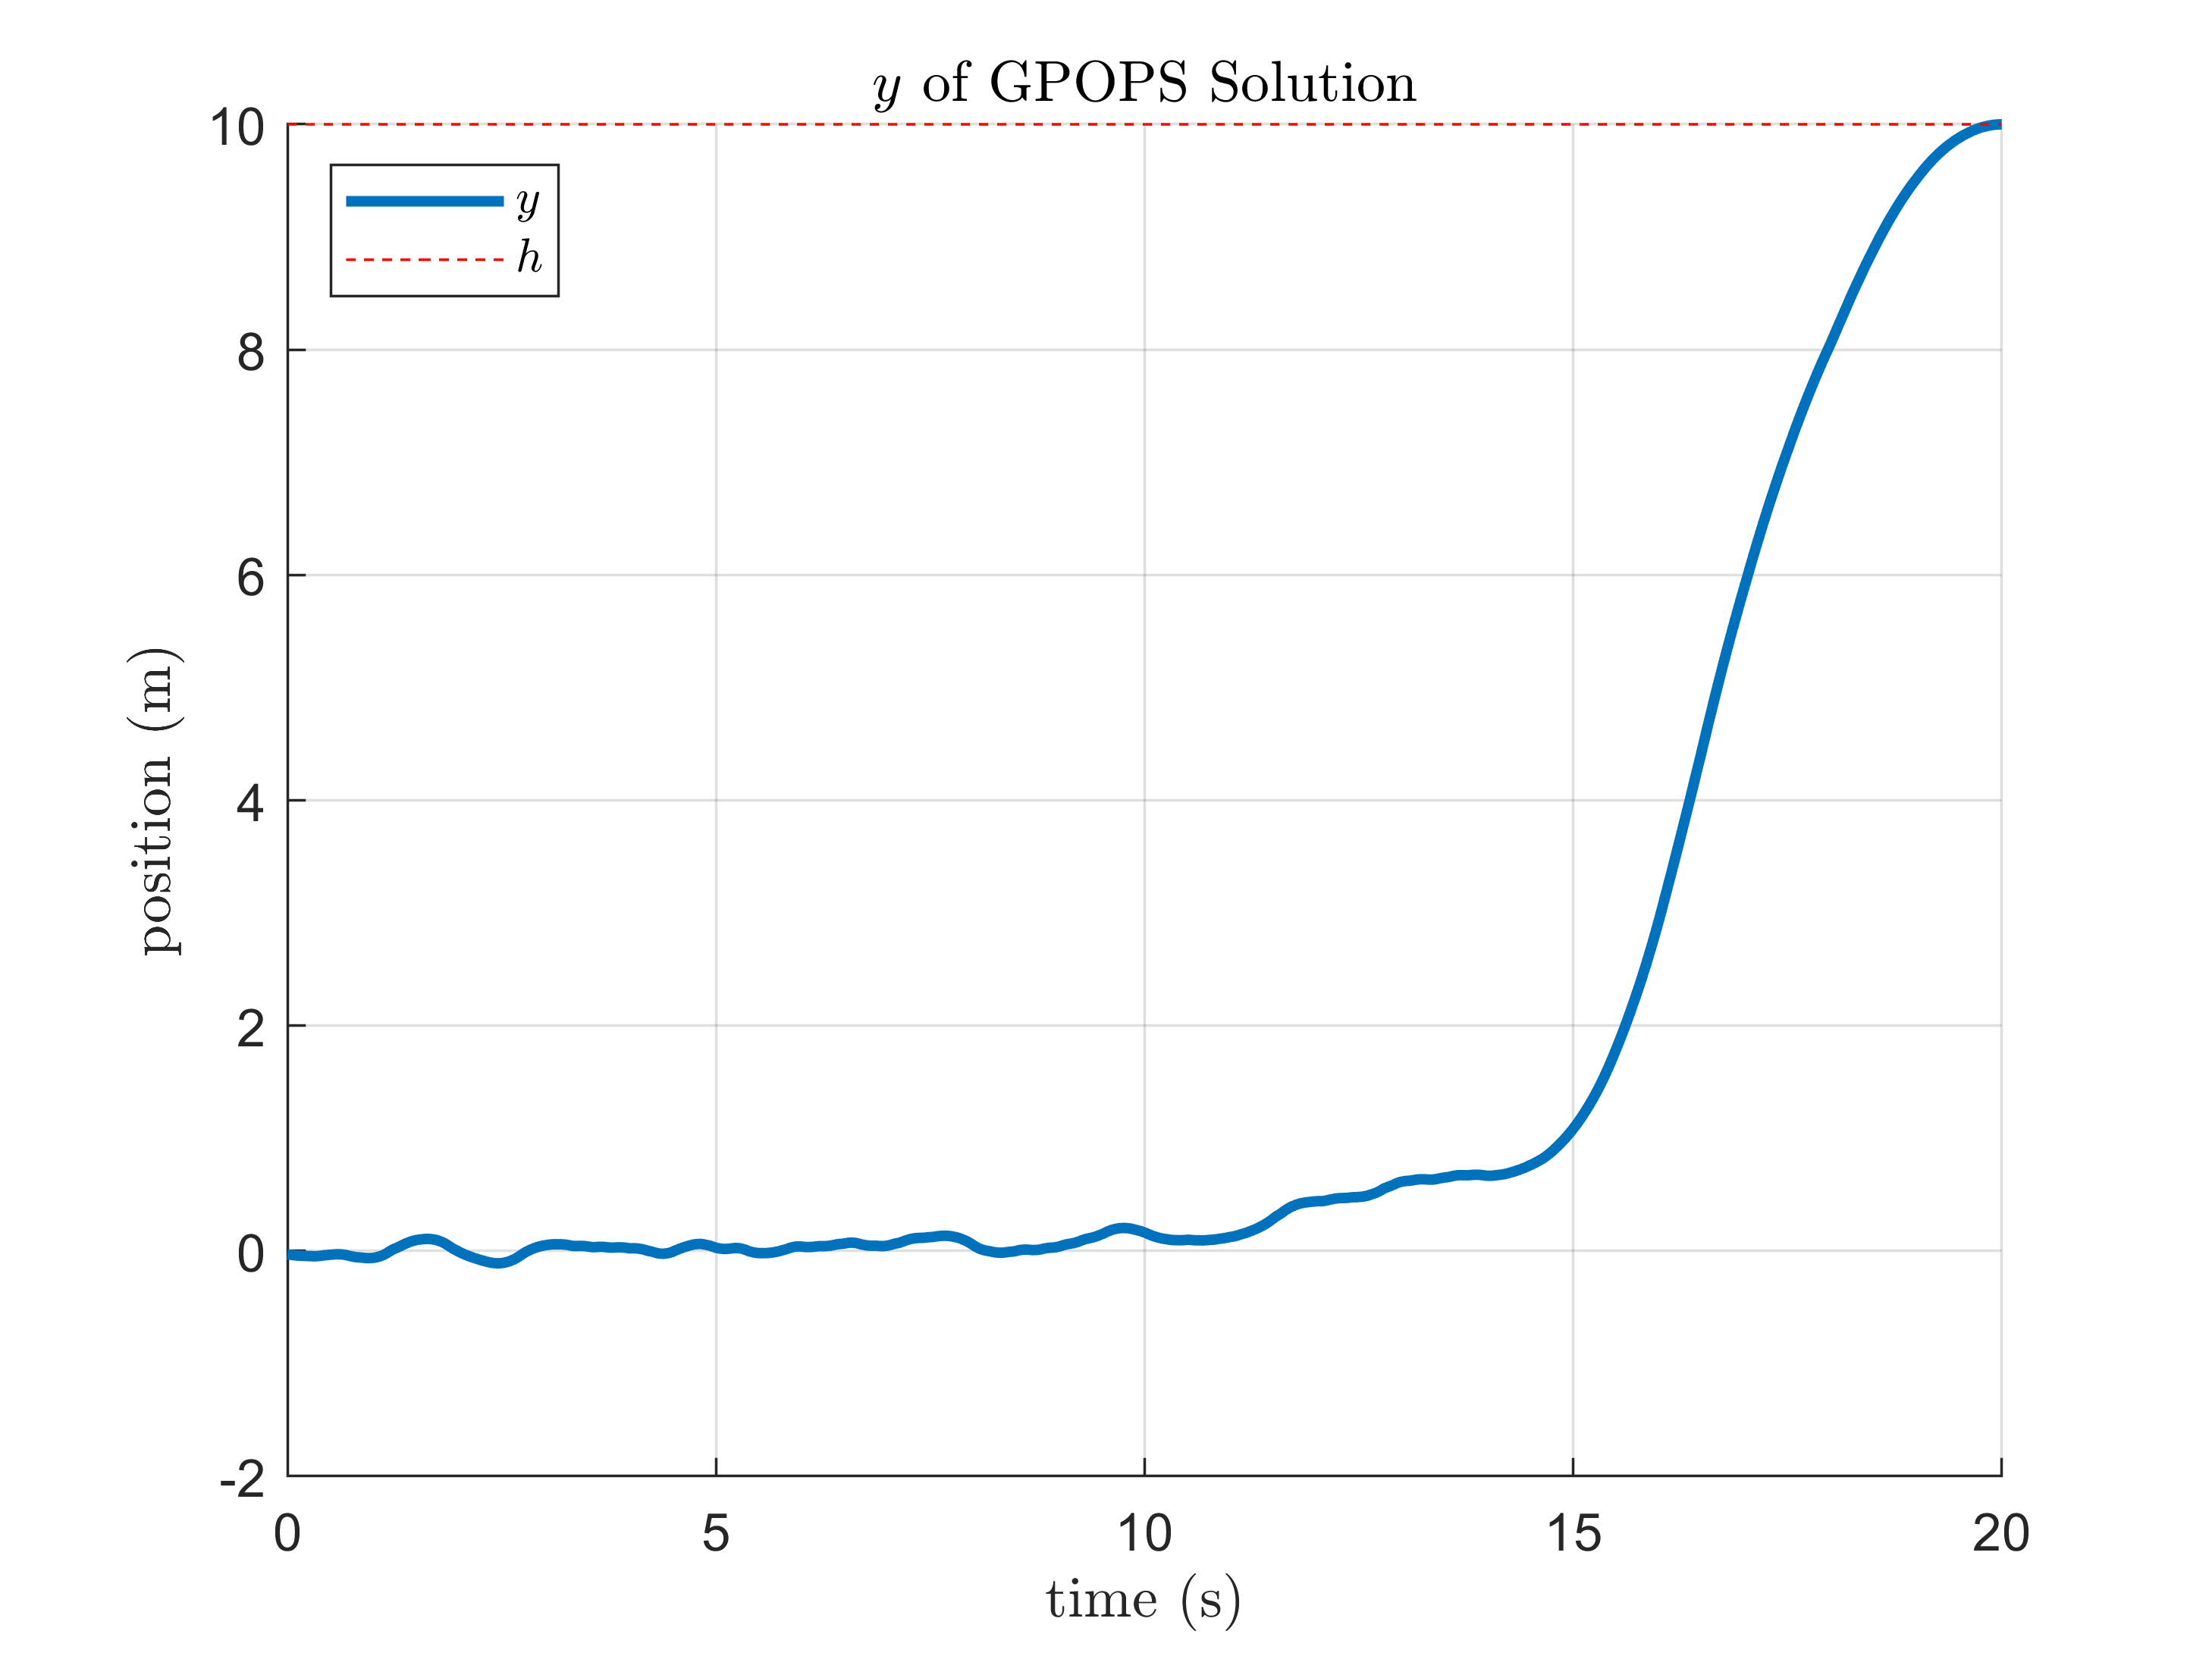
\includegraphics[width=\linewidth]{figures/SolY.png}
    \caption{Position in $y$-direction}
    \label{fig:ocp1_y}
  \end{subfigure}
  \caption{Position solution of the OCP using GPOPS-II}
  \label{fig:ocp1_sol}
\end{figure}

Fig. (\ref{fig:ocp1_y})에서 볼 수 있듯이, OCP의 목표 위치 $h$에 도달하는 것을 확인할 수 있다.
또한, Fig. (\ref{fig:ocp1_v}) 역시 OCP의 최종 속도 $v(T)$가 0으로 도달한 것을 확인할 수 있다.

\begin{figure}[ht]
    \centering
    \begin{subfigure}[b]{0.49\linewidth}
        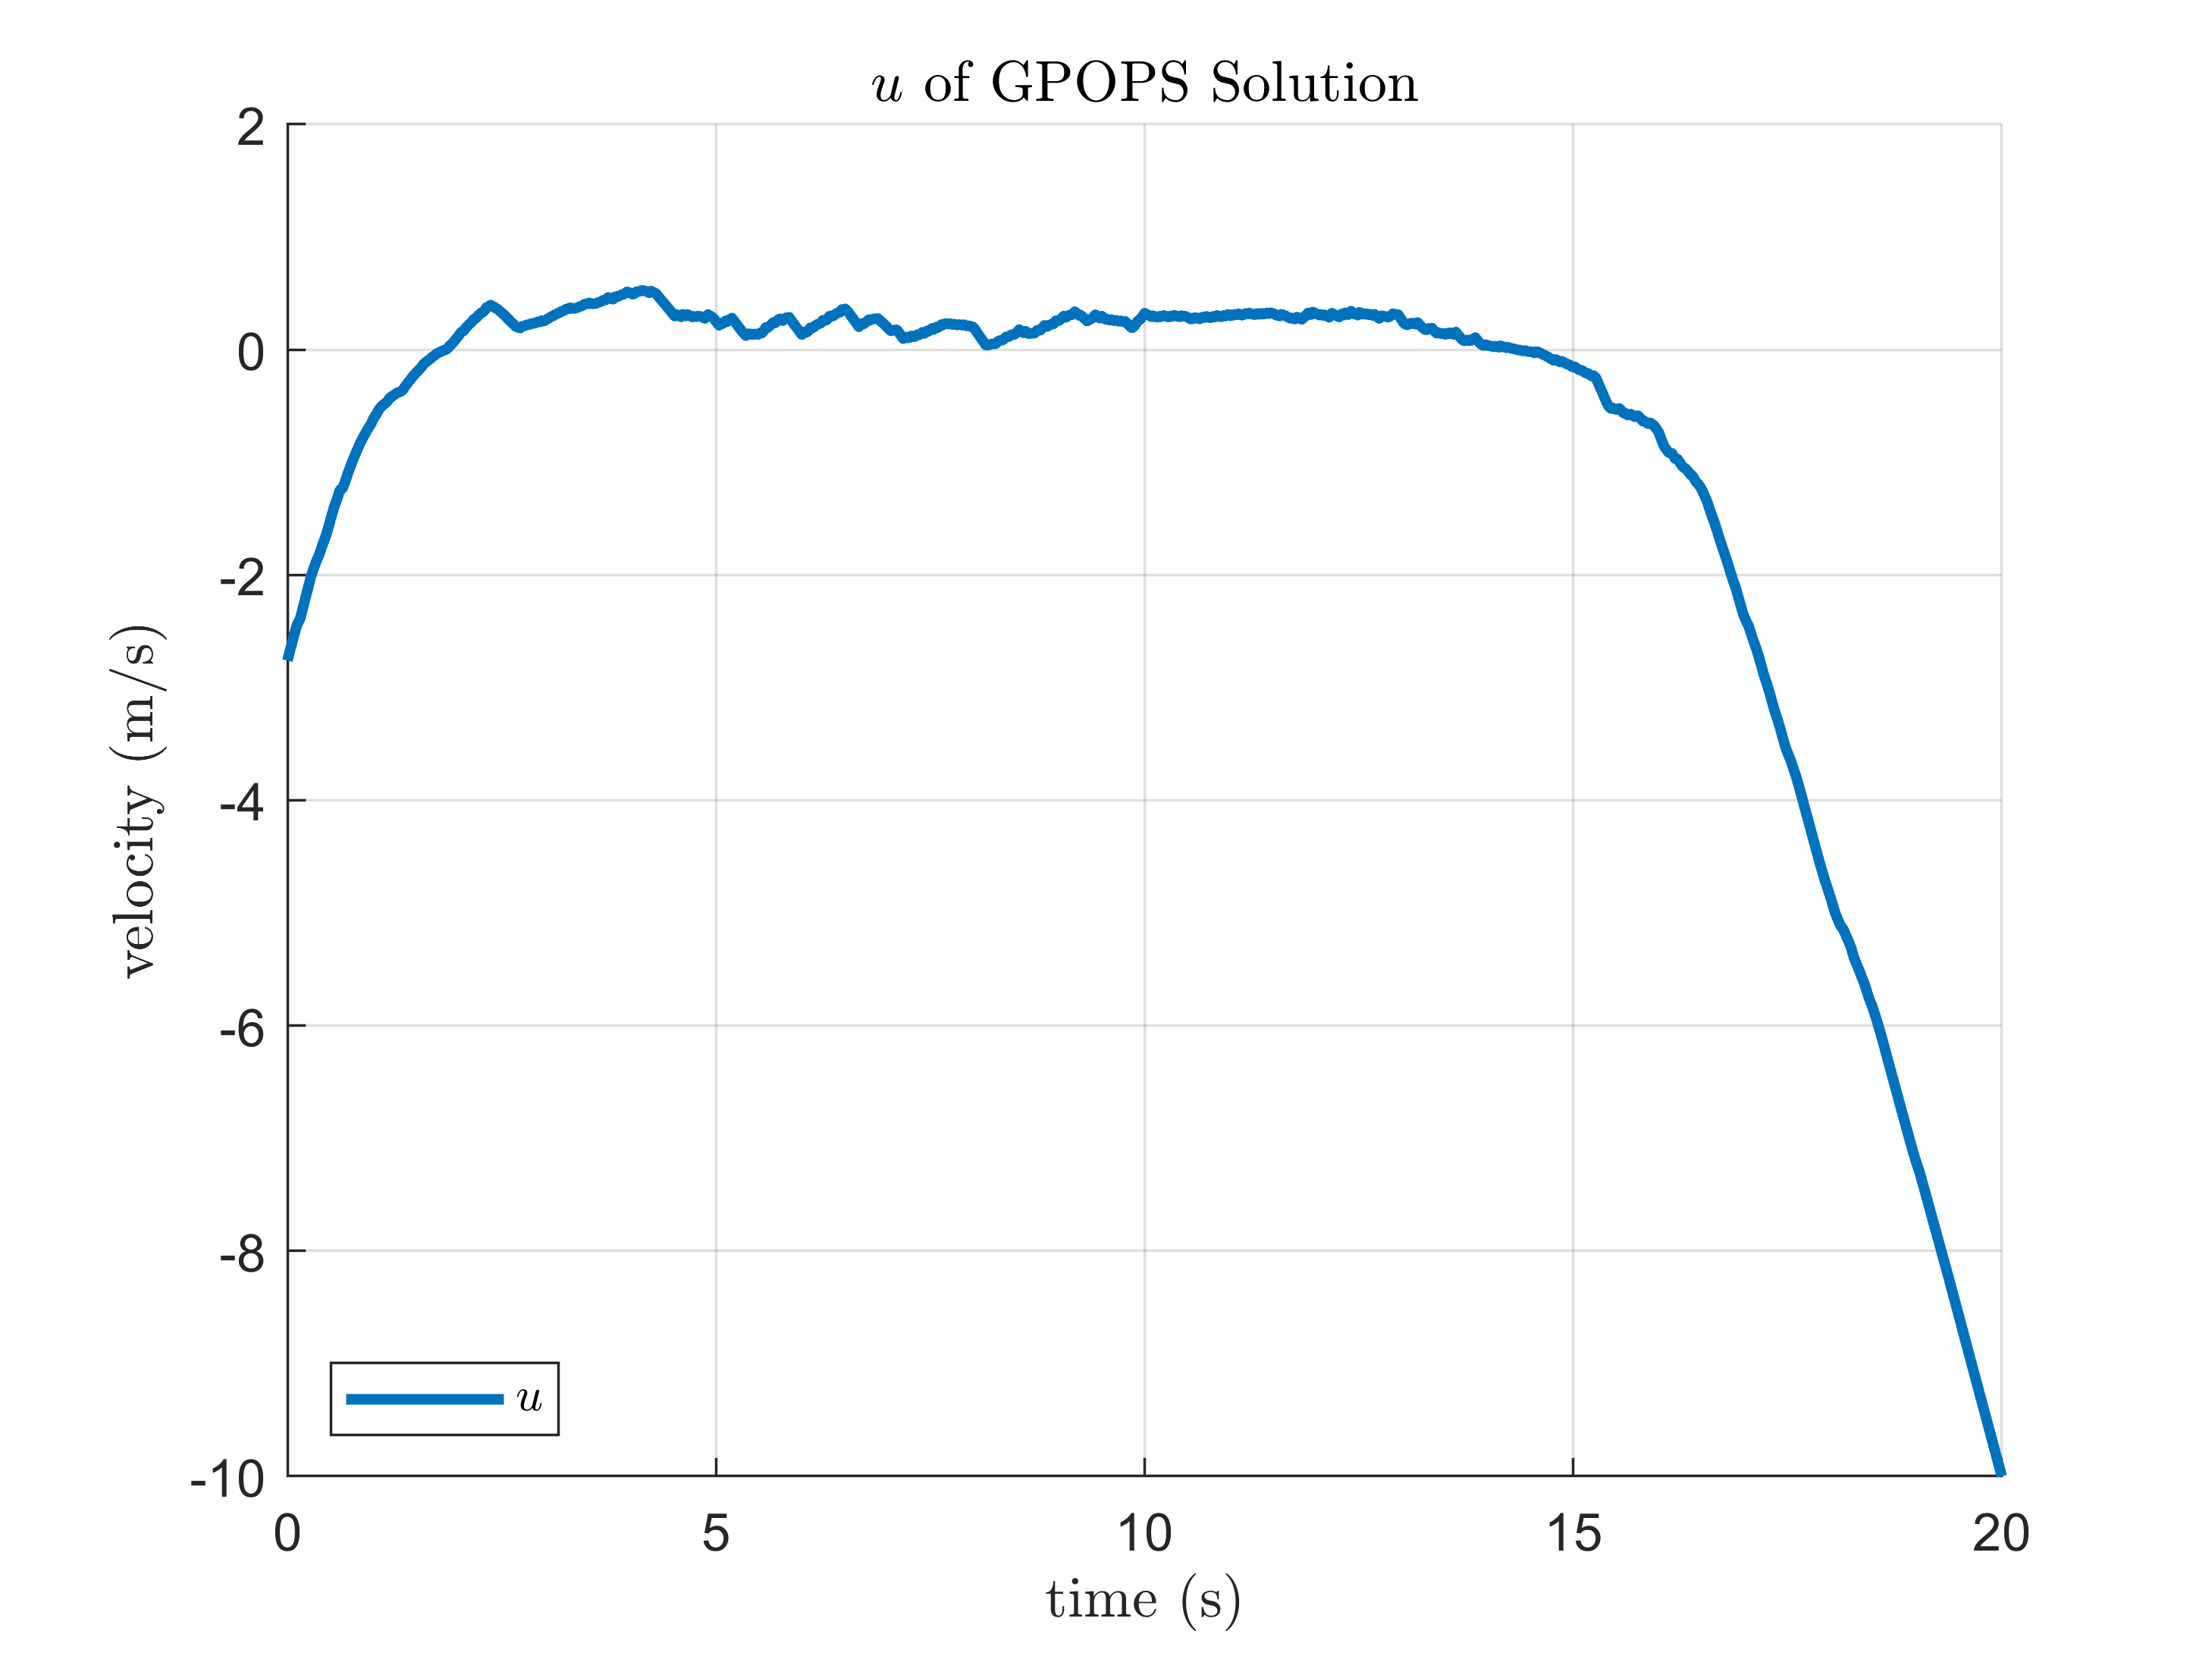
\includegraphics[width=\linewidth]{figures/SolU.png}
        \caption{Velocity in $x$-direction : $u$}
        \label{fig:ocp1_u}
    \end{subfigure}
    \hfill
    \begin{subfigure}[b]{0.49\linewidth}
        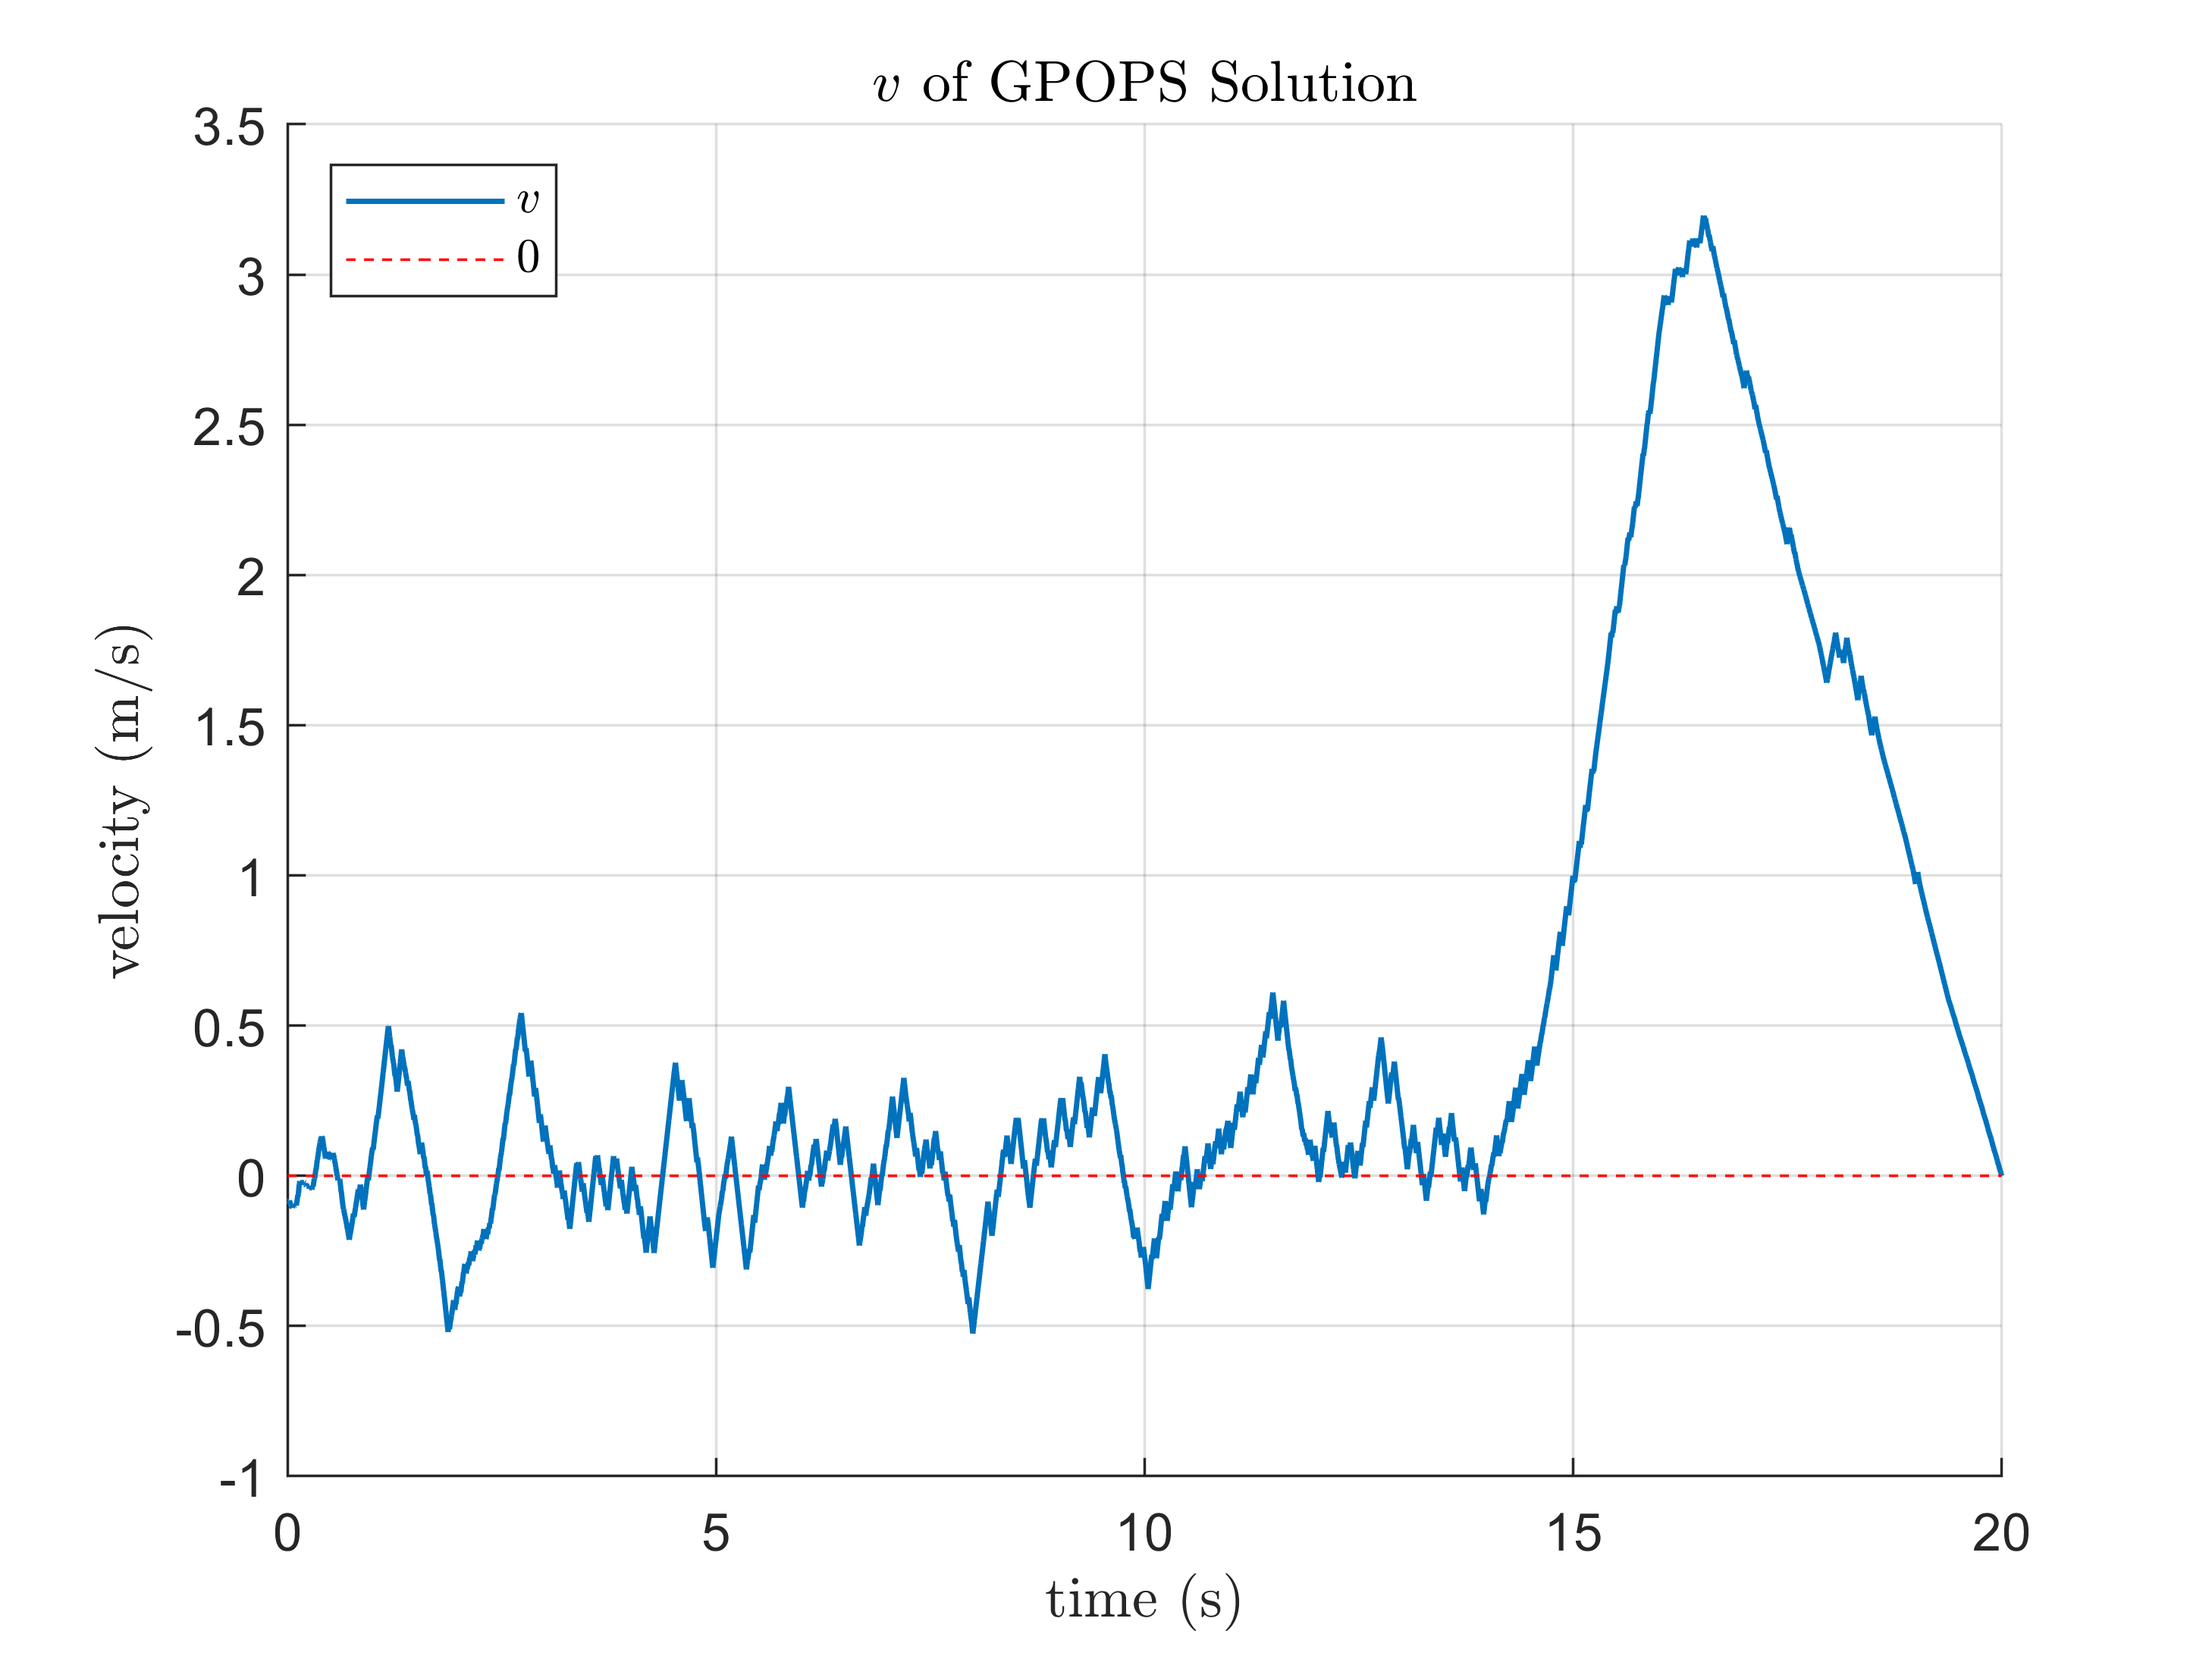
\includegraphics[width=\linewidth]{figures/SolV.png}
        \caption{Velocity in $y$-direction : $v$}
        \label{fig:ocp1_v}
    \end{subfigure}
    \caption{Velocity solution of the OCP using GPOPS-II}
    \label{fig:ocp1_vel}    
\end{figure}

GPOPS-II를 사용한 OCP의 solution에서, $x(0)$를 제외한 초기 상태들은 각각 $y(0) = -0.0302\,m$, $u(0) = -2.7604\,m/s$, $v(0) = -0.0842\,m/s$로 설정한 bound 내의 값들로 정의되었다.
GPOPS-II 알고리즘은 $J$를 최소화하기 위해 지정한 최종 시간 $T$를 모두 사용한 것을 확인할 수 있다.
앞서 언급했듯, objective function $J$는 최종 시간 $T$에서의 속도 $u(T)$를 최소화하는 것으로 정의된다.
따라서, Fig. (\ref{fig:ocp1_u}, \ref{fig:ocp1_obj})에서 볼 수 있듯, 최종 속도 $u(T)$는 지정한 bound인 $-10\,m/s$, objective function의 최솟값에 도달하도록 $\beta$가 조정됐음을 확인했다.
정의되지 않은 마지막 상태 $x(T)$는 $-18.6161\,m$로 설정한 bound 내의 값에서 시뮬레이션이 종료됐다.

\begin{figure}[ht]
    \centering
    \begin{subfigure}[b]{0.49\linewidth}
        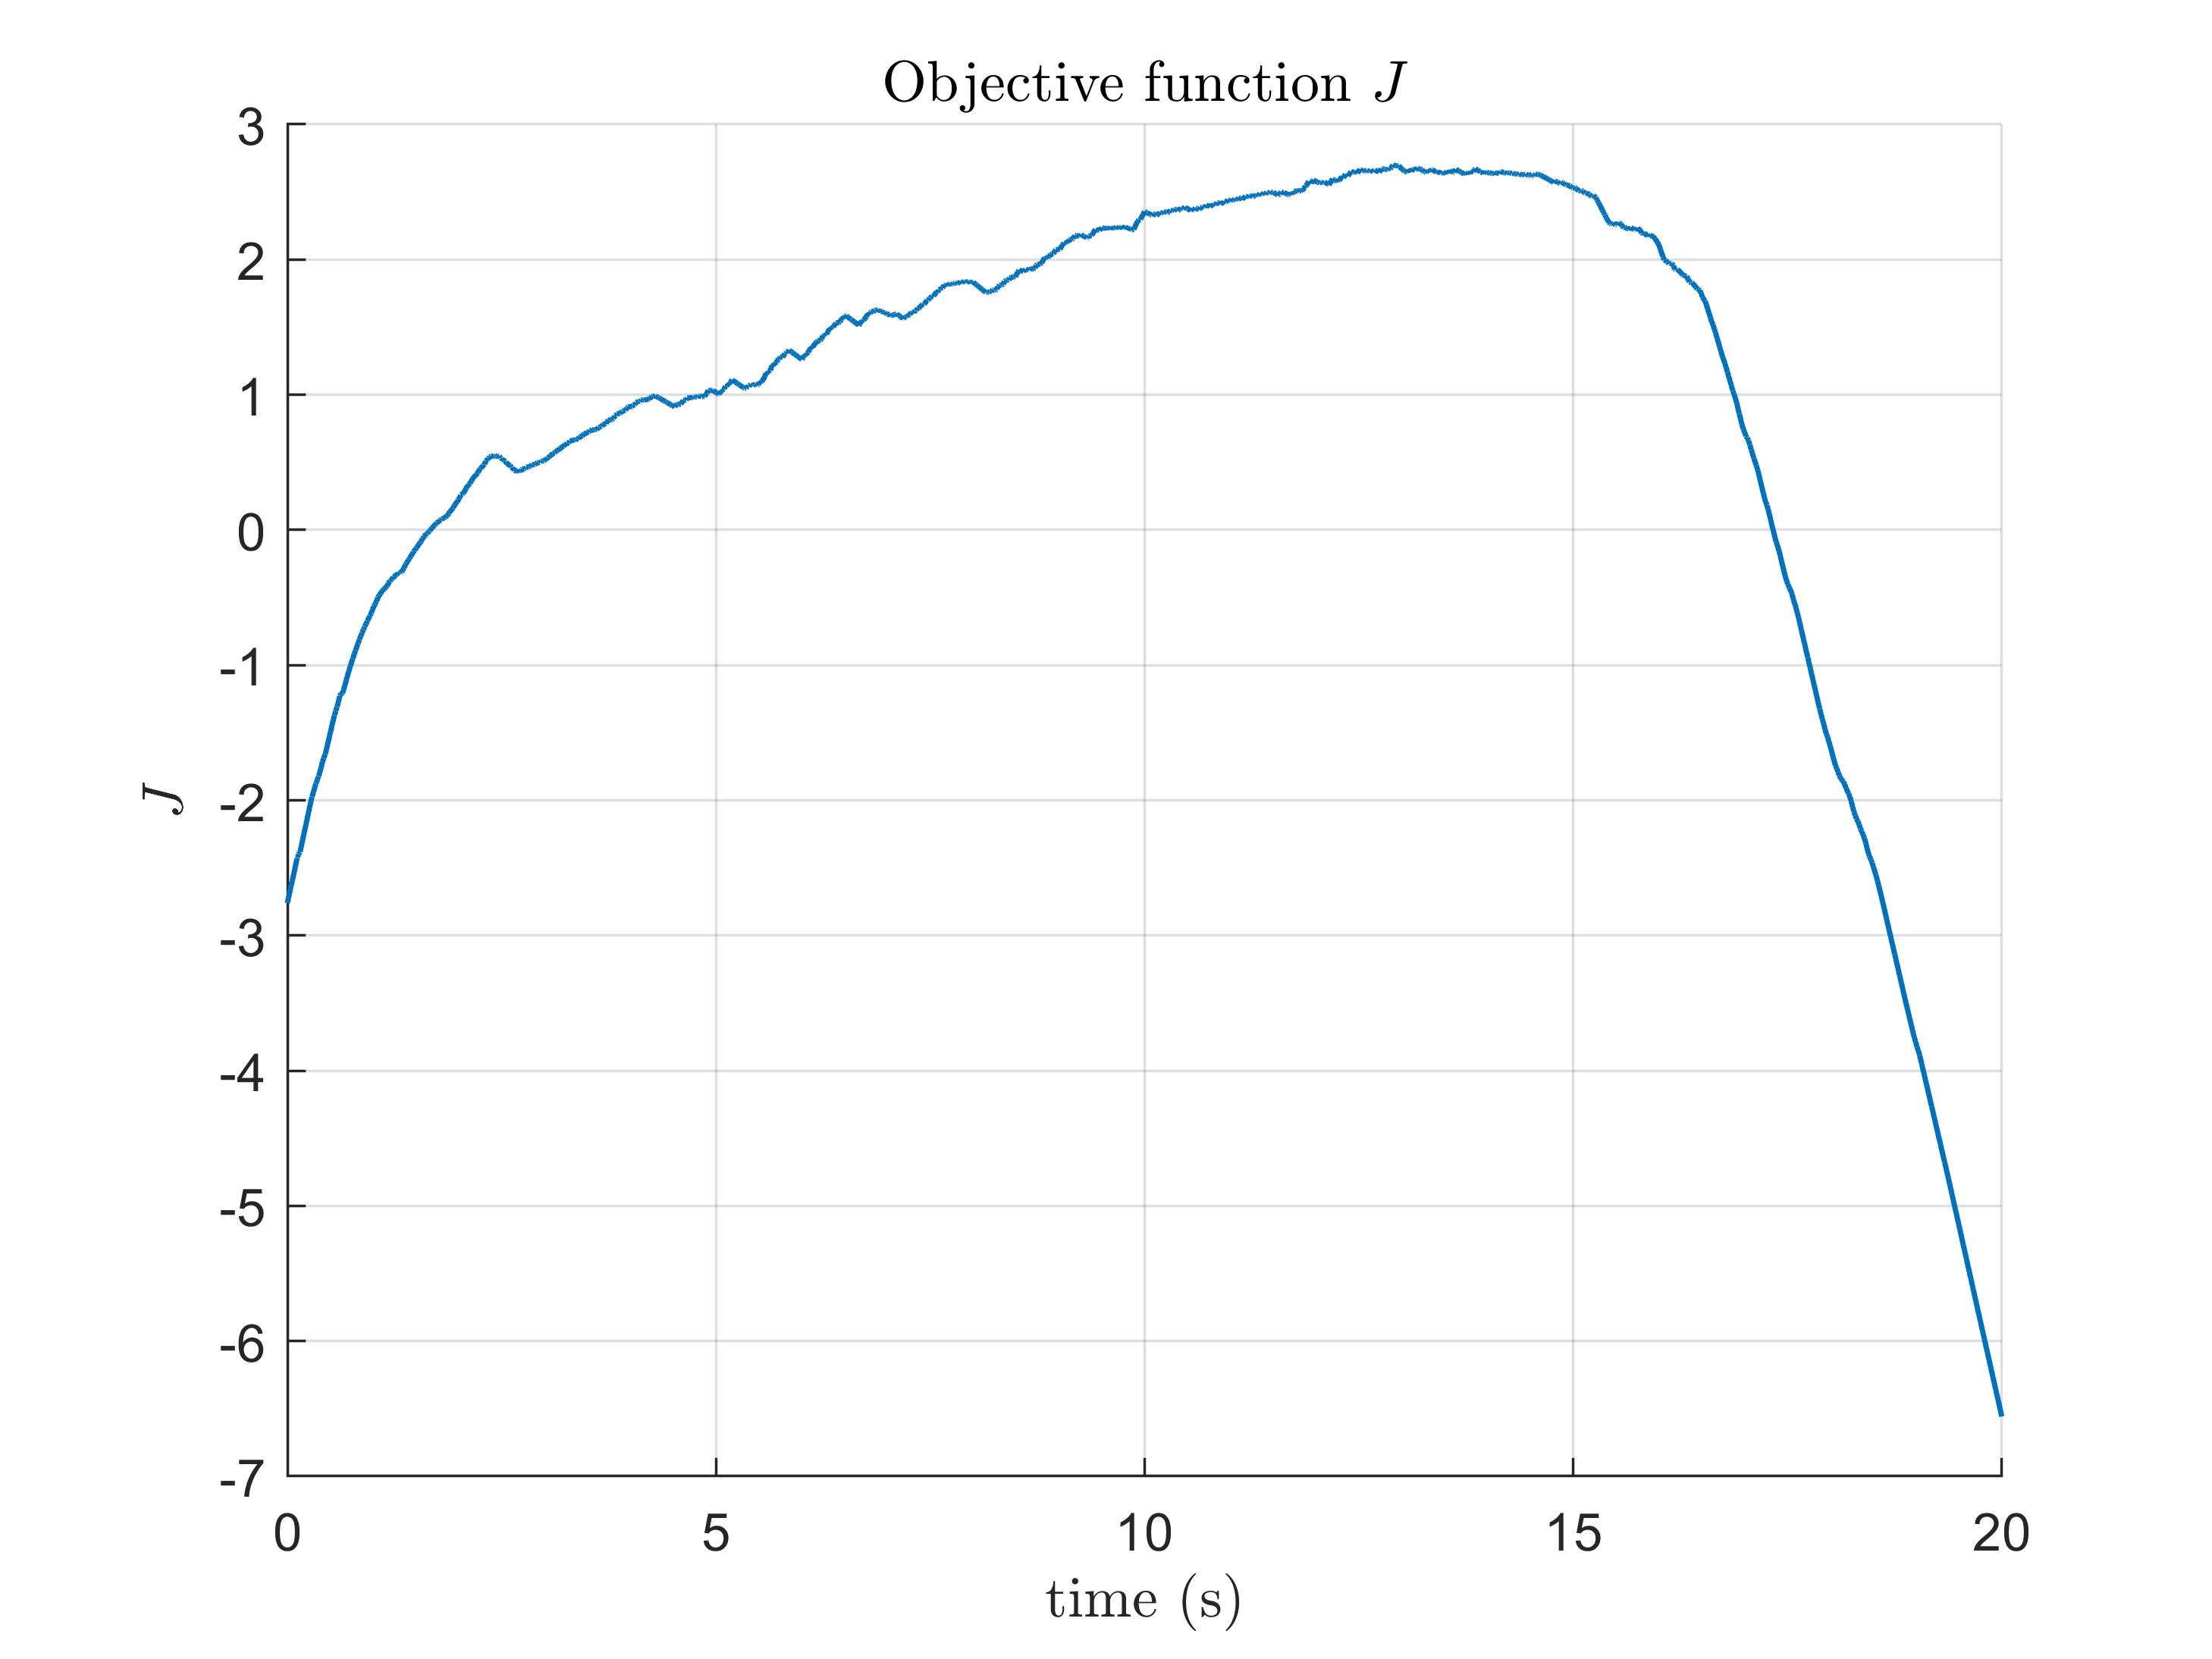
\includegraphics[width=\linewidth]{figures/ObjFcn.png}
        \caption{Objective function $J$}
        \label{fig:ocp1_obj}
    \end{subfigure}
    \hfill
    \begin{subfigure}[b]{0.49\linewidth}
        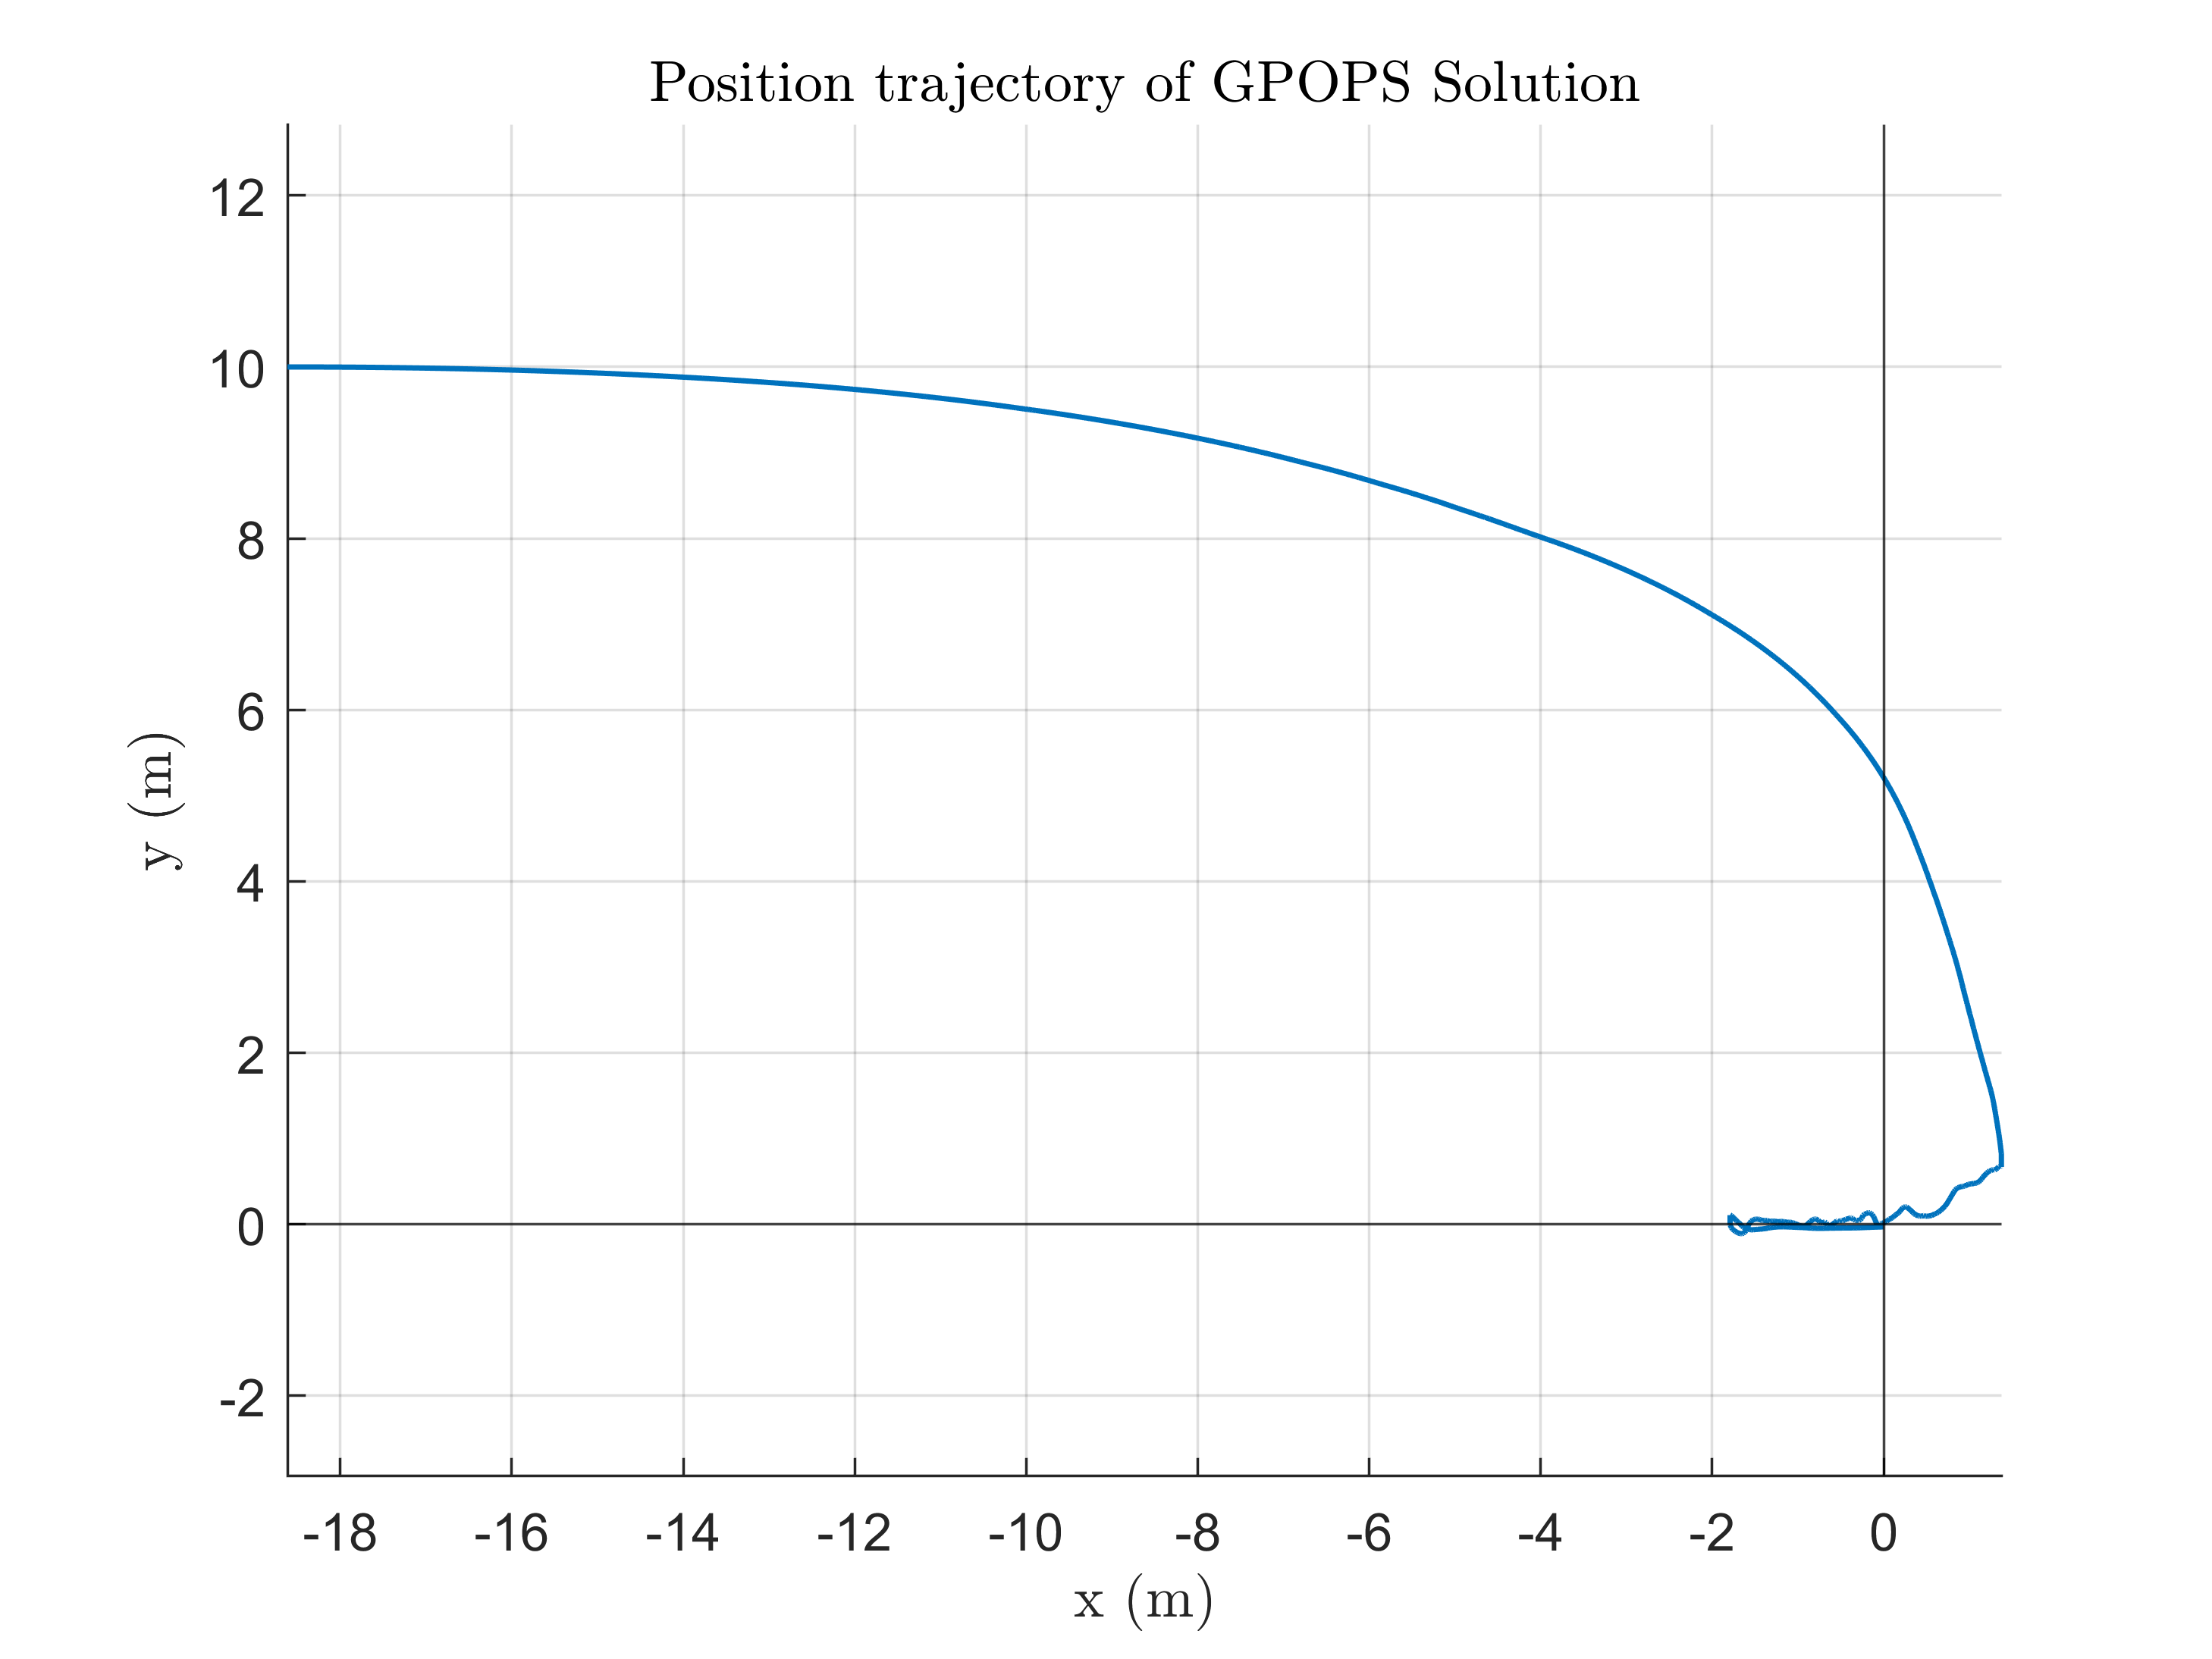
\includegraphics[width=\linewidth]{figures/TrajXY.png}
        \caption{Trajectory in $xy$-plane}
        \label{fig:ocp1_xy}
    \end{subfigure}
    \caption{Control and Trajectory solution of the OCP using GPOPS-II}
    \label{fig:ocp1_control}
\end{figure}

\begin{problem}{Problem [2]}{prob1-2}
Solve the above problem using "Direct Collocation Method"


\end{problem}

\begin{problem}{Problem [3]}{prob1-3}
Solve the above problem using indirect methods (quasi-linearizatin, differential correction, etc.)


\end{problem}

\bibliographystyle{apalike}
\bibliography{references}
\end{document}